\chapter{Implementation Design}
\label{ch:implementation}

\section{Design of the Physical Architecture}
\label{sec:phys}

\subsection{Selecting OpenStack Services}
The first decision when designing an OpenStack cloud deployment is about the services we need to have running.

For this thesis, I have chosen these five core services:
\begin{itemize}
  \item{OpenStack Identity (Keystone)}
  \item{OpenStack Image (Glance)}
  \item{OpenStack Compute (Nova)}
  \item{OpenStack Block Storage (Cinder)}
  \item{OpenStack Dashboard (Horizon)}
\end{itemize}

These services will be also required:
\begin{itemize}
  \item{SQL Database}
  \item{AMQP message broker}
\end{itemize}



\subsection{Selecting Specific Implementations}
The second decision is about technology. The most important is to choose a specific version of OpenStack. The OpenStack release chosen for this thesis will be Liberty. This is mostly because it is the  latest release at the time of writing the thesis.

I also need to choose an operating system platform that will run on the physical host machines. Choosing the right Linux distribution is important as there might be big differences in terms of available packages, stability, the lifecycle, and an option of commercial support. The target platform of deployment will be CentOS 7.2. CentOS is free and open source operating system based on the Red Hat Enterprise Linux platform. It uses the RPM packaging model and the OpenStack Liberty packages are included in the repositories. The system is stable, has a long lifecycle and potential migration to to a commercially supported environment would be easy, as it is based on the Red Hat Enterprise Linux platform.

OpenStack also needs an SQL database to store the state of the services, and it also might me used as a storage for the Identity service. In this deployment, it will be used in this way. I have chosen MariaDB because it is open source, widely used and handles memory well.

The next component is an AMQP broker. It is used by processes within the OpenStack service for communication, and it also might be used as a short-term storage by some networking plugins. For this particular deployment, I will use RabbitMQ because it is an open source solution and it is widely used in production environments. It is also well-supported by the OpenStack itself.

The last decision will be about storage backend for the OpenStack Block Storage service. I will use a local disk and an LVM technology. LVM is a robust and stable open source solution for storage that runs on commodity hardware, which is important especially for this testing environment.


\subsection{Physical architecture}

\begin{figure}[!h]
  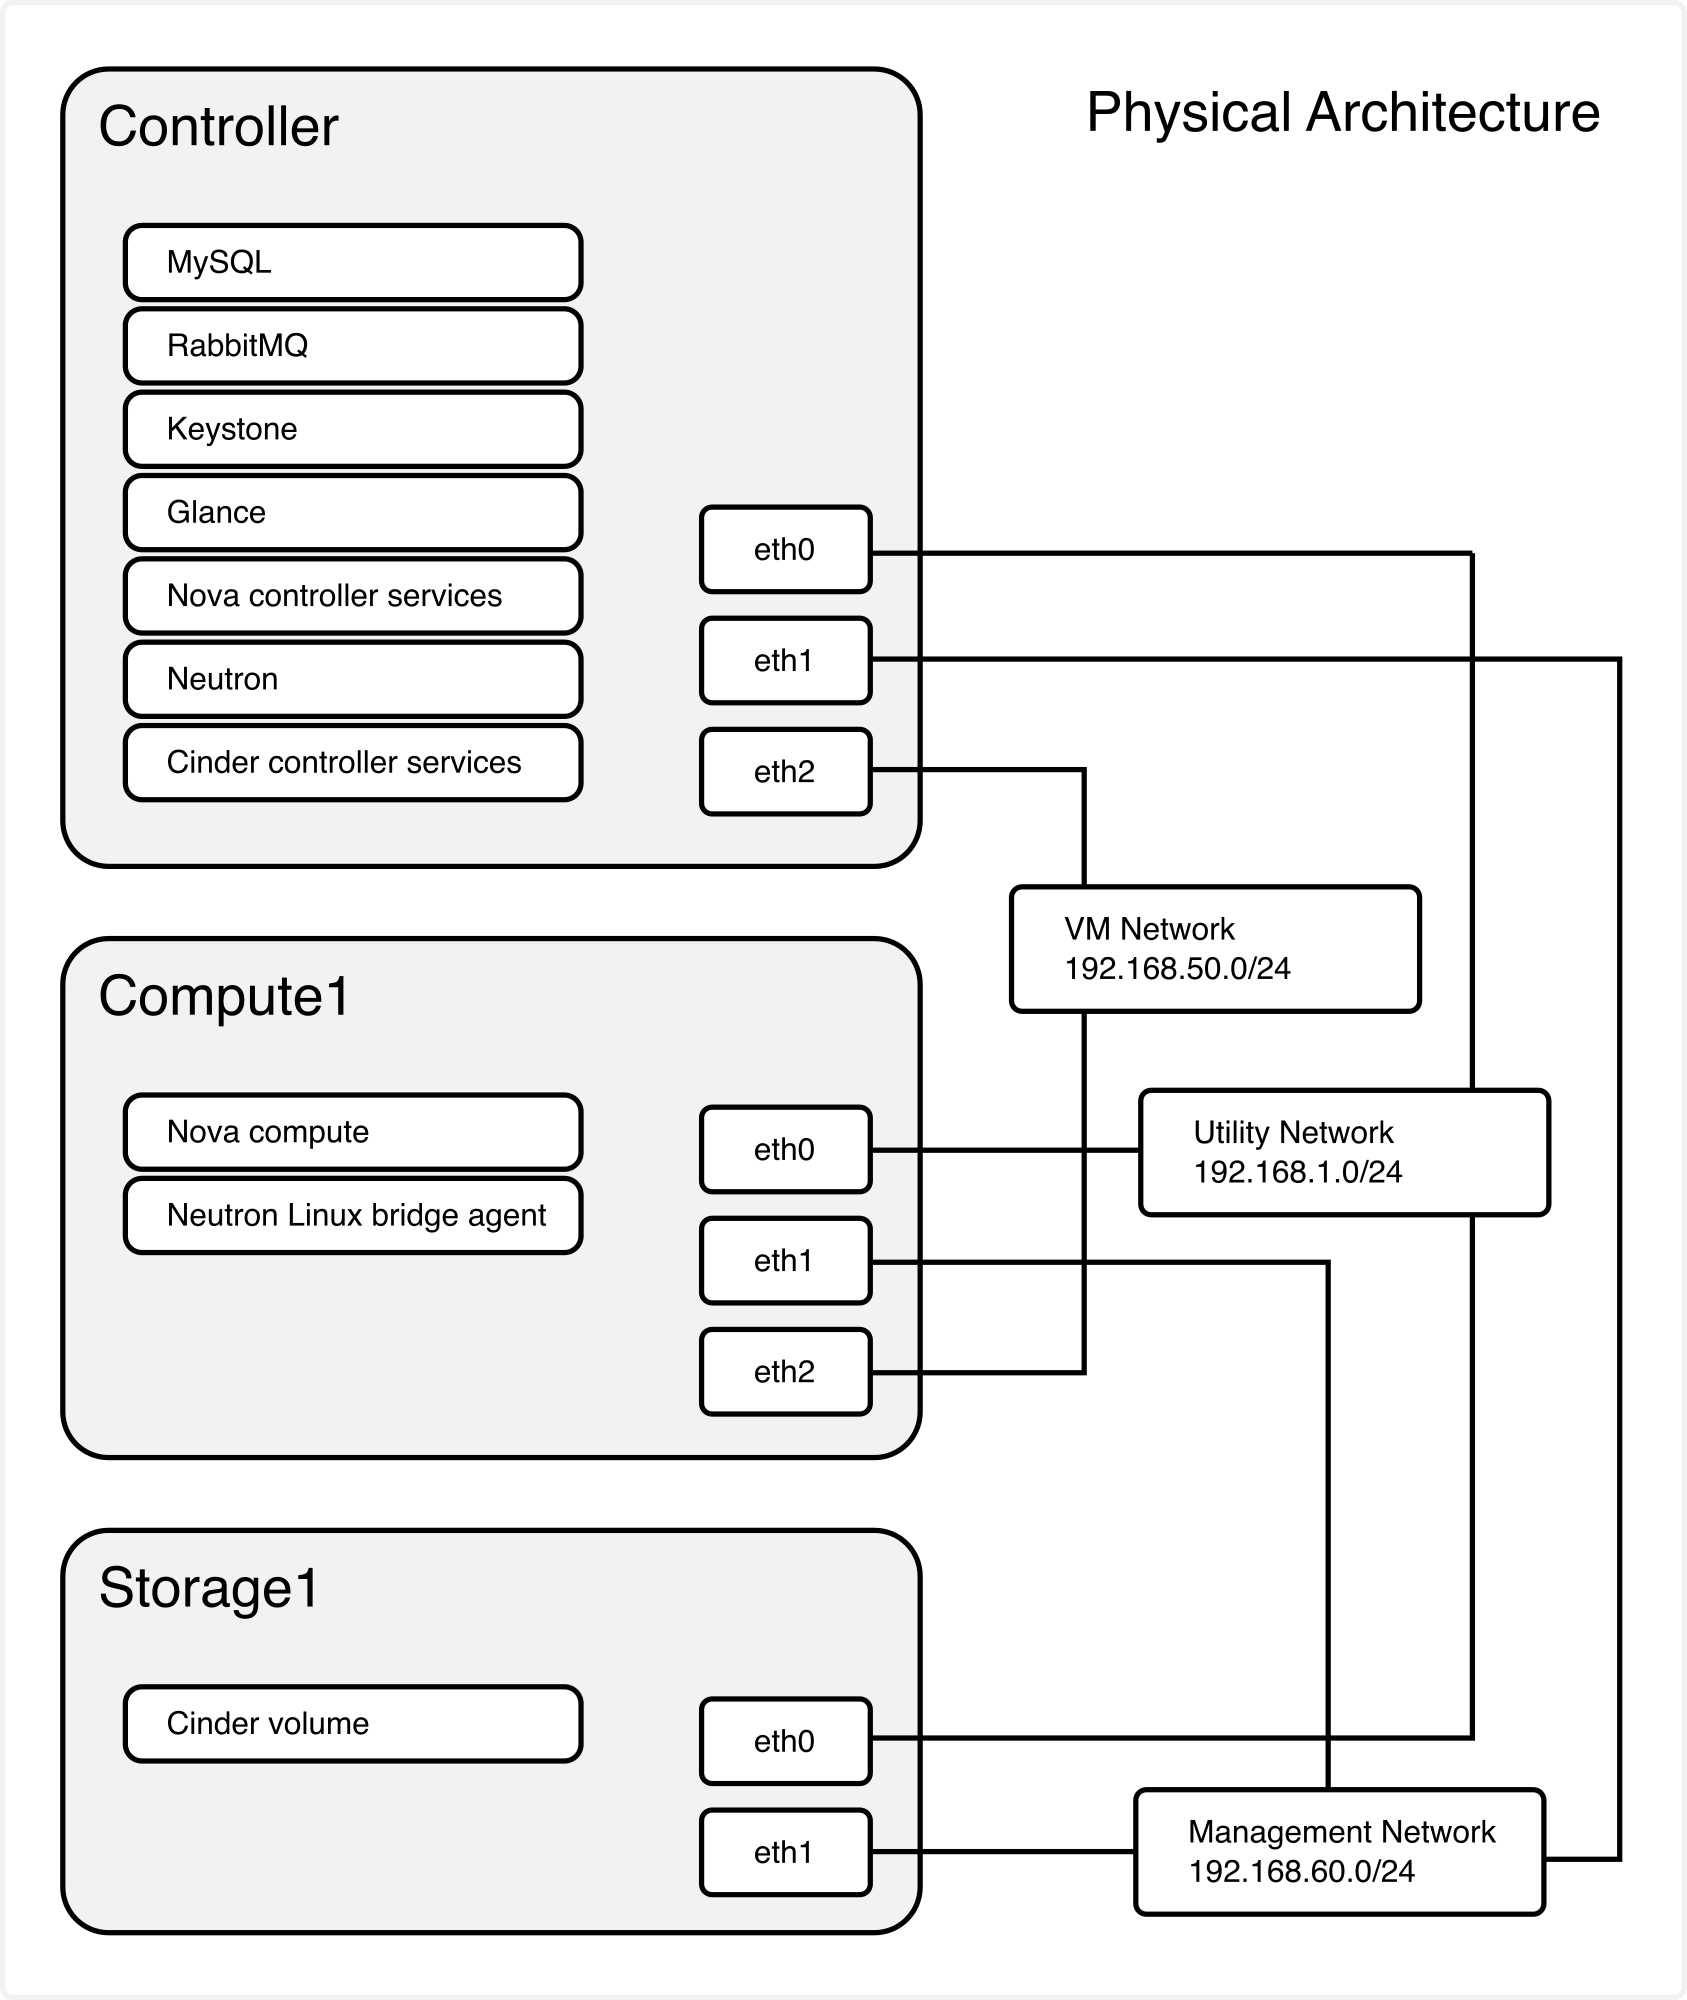
\includegraphics[width=\textwidth]{fig/my_architecture.png}
  \caption{OpenStack physical architecture design}
  \label{fig:openstack_physical_arch}
\end{figure}

\subsubsection*{Networks}
I have used three different networks in my architecture and each one have different purpose in the whole system. Their descriptions are as follows:
\begin{itemize}
  \item{\textbf{Utility Network} - This network is used the datacenter administrators to maintain the physical hosts. In this example it will also be used by Ansible to deploy the OpenStack and all other services.}
  \item{\textbf{Management Network} - This network is used by the OpenStack services to communicate with each other. It will also provide connectivity for the services to the MySQL database and the RabbitMQ Message Queue. All Keystone endpoints based on hostnames will also use this network. It will be also used to connect storage from Storage1 host to virtual machines running on the Compute1 host.}
  \item{\textbf{VM Network} - This network is used to provide outside connectivity to the virtual machines running on the compute node.}
\end{itemize}
It is also important to note that the eth2 interfaces on Controller and Compute1 hosts will use special configuration without an IP address and will be attached to virtual network bridges. Their specific configuration will be mentioned later in the text.



\section{Design of the Ansible Playbook}
\subsection{Ansible Roles}
The services will be installed on the target hosts using Ansible roles. Roles offer flexibility in a way, that each role can be installed separately on a given host, or, if needed, on multiple hosts. These roles can be then reused to deploy a different physical architectures.

All roles use handlers to restart services in case of a configuration change. All roles are also designed to be idempotent.

\subsubsection*{Role \texttt{sql-database}}
The role sql-database will deploy a MariaDB database on the target host. It will set the root password accordingly and will also remove the anonymous user as well as the test database.

The following packages will be installed:
\begin{itemize}
\item{\texttt{mariadb}}
\item{\texttt{mariadb-server}}
\item{\texttt{MySQL-python}}
\end{itemize}

And the following MariaDB service will be enabled and started:
\begin{itemize}
\item{\texttt{mariadb}}
\end{itemize}

\subsubsection*{Role \texttt{rabbit}}
The rabbit role will deploy a RabbitMQ message broker on the target host. It will also create a new user needed for the OpenStack deployment.

The following package will be installed:
\begin{itemize}
  \item{\texttt{rabbitmq-server}}
\end{itemize}

And the following RabbitMQ service will be enabled and started:
\begin{itemize}
  \item{\texttt{rabbitmq-server}}
\end{itemize}

\subsubsection*{Roles \texttt{controller-basic} and \texttt{compute-basic}}
The roles controller-basic and compute-basic enable the OpenStack Liberty repository for CentOS and install the SELinux package. These roles are the first that should be run before any other openstack roles.

These roles will install these two packages:
\begin{itemize}
  \item{\texttt{python-openstackclient}}
  \item{\texttt{openstack-selinux}}
\end{itemize}

\subsubsection*{Role \texttt{keystone}}
The keystone role will install the OpenStack Identity service, codename Keystone, on the target host. It requires an SQL database to be running on the network. The example in this thesis will run the database on the controller node.

The role will create a database for the Keystone service called keystone.

This role will install the following packages:
\begin{itemize}
  \item{\texttt{openstack-keystone}}
  \item{\texttt{httpd}}
  \item{\texttt{mod\_wsgi}}
  \item{\texttt{memcached}}
  \item{\texttt{python-memcached}}
  \item{\texttt{python-keystoneclient}}
\end{itemize}
And will enable and start the httpd service on the target host.



\subsubsection*{Role \texttt{glance}}
The glance role will install the OpenStack Image service, codename Glance, on the target host. It requires an SQL database, and the OpenStack Identity service to be running on the network. The example in this thesis will run both on the controller node.

The role will create a database for the Glance service called glance, and registers the Glance service and creates endpoints in the Keystone service.

Glance supports several backends for storing images. This role uses local filesystem to do so. Metadata about the images will be stored in the SQL database running on the controller node.

This role will install the following packages:
\begin{itemize}
  \item{\texttt{openstack-glance}}
  \item{\texttt{python-glance}}
  \item{\texttt{python-glanceclient}}
\end{itemize}
And the two following services will be enabled and started:
\begin{itemize}
  \item{\texttt{openstack-glance-api}}
  \item{\texttt{openstack-glance-registry}}
\end{itemize}


\subsubsection*{Role \texttt{nova-controller}}
The nova-controller role will install some parts of the OpenStack Compute service, codename Nova, on the target host. It requires an SQL database, RabbitMQ message bus, and the OpenStack Identity service to be running on the network. The example in this thesis will run all these services on the controller node.

The role will create a database for the Nova service called nova, and registers the Nova service and creates endpoints in the Keystone service.

Besides the standard configurations like setting hostname, configuration of database, and message bus access, the Nova service will be configured to use the OpenStack Networking (as opposed to legacy Nova networking) with the Linux bridge driver.

This role will install the following packages:
\begin{itemize}
  \item{\texttt{openstack-nova-api}}
  \item{\texttt{openstack-nova-cert}}
  \item{\texttt{openstack-nova-conductor}}
  \item{\texttt{openstack-nova-console}}
  \item{\texttt{openstack-nova-novncproxy}}
  \item{\texttt{openstack-nova-scheduler}}
  \item{\texttt{python-novaclient}}
\end{itemize}
And the following services will be enabled and started:
\begin{itemize}
  \item{\texttt{openstack-nova-api}}
  \item{\texttt{openstack-nova-cert}}
  \item{\texttt{openstack-nova-consoleauth}}
  \item{\texttt{openstack-nova-scheduler}}
  \item{\texttt{openstack-nova-conductor}}
  \item{\texttt{openstack-nova-novncproxy}}
\end{itemize}

\subsubsection*{Role \texttt{nova-compute}}
The nova-compute role will install the nova-compute process of the OpenStack Compute service, codename Nova, on the target host. It requires the RabbitMQ message bus to be running on the network. The example in this thesis will run it on the controller node.

The role will configure an access to the necessary Nova processes installed by the nova-controller role, and will also configure Nova to use the OpenStack Networking with the Linux bridge driver.

It will also configure the hypervisor. This role uses the libvirt provider using QEMU. This is because VirtualBox, which is used for testing the deployment, does not support nested virtualisation, so KVM can not be used.

This role will install these two packages:
\begin{itemize}
  \item{\texttt{openstack-nova-compute}}
  \item{\texttt{sysfsutils}}
\end{itemize}
And will start and enable the two following services:
\begin{itemize}
  \item{\texttt{libvirtd}}
  \item{\texttt{openstack-nova-compute}}
\end{itemize}

\subsubsection*{Role \texttt{neutron-controller}}
The neutron-controller role will install the OpenStack Networking service, codename Neutron, on the target host. It requires an SQL database, RabbitMQ message bus, and the OpenStack Identity service to be running on the network. The example in this thesis will run all these services on the controller node. This role also requires the nova-compute role to be run on the same host before.

The role will create a database for the Neutron service called neutron, and registers the Neutron service and creates endpoints in the Keystone service.

The OpenStack Networking service uses plug-ins and agents for the actual networking functionality. This role will use:
\begin{itemize}
  \item{\texttt{Modular Layer 2 (ML2) plugin}}
  \item{\texttt{Linux bridge agent}}
  \item{\texttt{Layer-3 agent}}
  \item{\texttt{DHCP agent}}
\end{itemize}
This setup will allow to create tenant networks as well as public provider networks.

The ML2 plugin will be configured to use the Linux bridge technology and VXLAN to create the tenant networks.

The Linux bridge agent will be configured to use VXLAN for the tenant networks and iptables firewall driver to manage security groups.

The layer-3 agent will be configured to use the Linux bridge driver and to support multiple external networks.

The DHCP agent will be also configured to use the Linux bridge driver and the MTU is set to 1450 bytes. This is because the VXLAN includes additional packet header and virtual machines running in the cloud use the default MTU of 1500 bytes. Using this settings, the virtual machines will use the smaller MTU, which would allow space for the additional header.

Finally, the Nova service will be configured to use the OpenStack Networking service, installed by this role.

This role will install the following packages:
\begin{itemize}
  \item{\texttt{openstack-neutron}}
  \item{\texttt{openstack-neutron-ml2}}
  \item{\texttt{openstack-neutron-linuxbridge}}
  \item{\texttt{python-neutronclient}}
  \item{\texttt{ebtables}}
  \item{\texttt{ipset}}
\end{itemize}
It will restart this Nova service:
\begin{itemize}
  \item{\texttt{openstack-nova-api}}
\end{itemize}
And the following services will be started and enabled:
\begin{itemize}
  \item{\texttt{neutron-server}}
  \item{\texttt{neutron-linuxbridge-agent}}
  \item{\texttt{neutron-dhcp-agent}}
  \item{\texttt{neutron-metadata-agent}}
  \item{\texttt{neutron-l3-agent}}
\end{itemize}


\subsubsection*{Role \texttt{neutron-compute}}
The neutron-compute role will install the Linux bridge agent of the OpenStack Networking service, codename Neutron, on the target host.  It requires the RabbitMQ message bus to be running on the network. The example in this thesis will run it on the controller node. It also require the role nova-compute to be run on the same host before.

This role will configure the Linux bridge agent to use the correct network interface as a public interface, enables VXLAN for the tenant networks, and configures iptables as a firewall driver to manage security groups.

It will also configure the Nova service to use the OpenStack Networking.

This role will install the following packages:
\begin{itemize}
  \item{\texttt{openstack-neutron}}
  \item{\texttt{openstack-neutron-linuxbridge}}
  \item{\texttt{ebtables}}
  \item{\texttt{ipset}}
\end{itemize}
It will restart this Nova service:
\begin{itemize}
  \item{\texttt{openstack-nova-compute}}
\end{itemize}
And also the Linux bridge agent service will be started and enabled:
\begin{itemize}
  \item{\texttt{neutron-linuxbridge-agent}}
\end{itemize}


\subsubsection*{Role \texttt{dashboard}}
The dashboard role will install the OpenStack Dashboard service, codename Horizon, on the target host. The Dashboard service installed by this role uses the Apache httpd web server.

It will install the following packages:
\begin{itemize}
  \item{\texttt{openstack-dashboard}}
  \item{\texttt{httpd}}
  \item{\texttt{memcached}}
\end{itemize}
And the following services will be started and enabled:
\begin{itemize}
  \item{\texttt{httpd}}
  \item{\texttt{memcached}}
\end{itemize}




\subsection{Applying Roles to the Hosts}

The Ansible playbook will apply the roles to the target hosts to match the physical architecture, which has been designed in \ref{sub:phys}

The list of nodes and playbooks that will be applied to them:

\subsubsection{Controller node}

\begin{itemize}
  \item{Role controller-basic}
  \item{Role rabbit}
  \item{Role sql-database}
  \item{Role dashboard}
  \item{Role glance}
  \item{Role keystone}
  \item{Role neutron-controller}
  \item{Role nova-controller}
  \item{Role cinder-controller}
\end{itemize}

\subsubsection{Compute node}

\begin{itemize}
  \item{Role compute-basic}
  \item{Role neutron-compute}
  \item{Role nova-compute}
\end{itemize}

\subsubsection{Storage node}

\begin{itemize}
  \item{Role storage-basic}
  \item{Role cinder-storage}
\end{itemize}
